\documentclass{beamer}
\usepackage{times, amsthm, amsmath, amssymb, cancel, changepage, graphicx, lipsum, fancyhdr, mathabx, enumitem,caption, subcaption}
\usetheme{CambridgeUS}
\usecolortheme{seagull}
\usefonttheme{serif}
\definecolor{navy}{RGB}{0, 0, 128} 
\setbeamercolor{frametitle}{fg=navy}
\setbeamercolor{title}{fg=navy}
\setbeamerfont{frametitle}{series=\bfseries}
\setbeamerfont{title}{series=\bfseries}


\title{Lecture 7: Limits, Continuity, and Derivatives in Several Variables}
\date{September 17, 2019}

\begin{document}
	
\frame{\titlepage}


\begin{frame}
\frametitle{Functions of Two Variables}
\begin{figure}
	\centering
	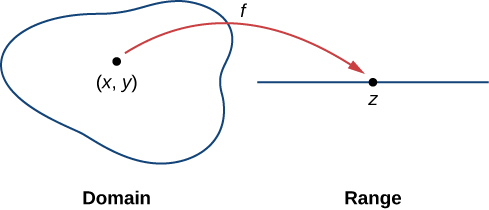
\includegraphics[height=.25\textheight]{function_map.jpg}\\
	\hspace*{10pt}\hbox{\thinspace{\tiny\itshape BC Open Textbooks}}
\end{figure}

A function of two variables is a rule that assigns to each ordered pair $(x,y)$ in $D$ a unique real nuber denote by $f(x,y)$. The set $D$ is the domain of $f$ and its range is the set of values that $f$ takes on.

\vspace{6pt}
\textbf{Examples:}
\begin{itemize}
	\item[(a)] Find the domain of $f$ and $g$ and evaluate $f(2,5)$, $f(1,2)$, $g(3,2)$
	$$f(x,y) = \frac{xy-5}{2 \sqrt{y-x^2}}, \, g(x,y) \frac{\sqrt{x+y+1}}{x-1}$$
\end{itemize}
\end{frame}


\begin{frame}
\frametitle{Limits in Two Variables}
Let $f$ be a function of a two variables defined on ad isk with center at $(a,b)$ expect possibly at $(a,b)$ itself. The limit of $f(x,y)$ as $(x,y)$ approaches $(a,b)$ is given by 
$$\lim\limits_{(x,y) \to (a,b)} f(x,y) = L$$
 if $\forall \epsilon > 0, \exists \delta > 0 \mbox{ s.t. } |f(x,y) - L| < \epsilon$
 
\vspace{12pt}
\textbf{Examples:}
\begin{itemize}
	\item[(a)] $\lim\limits_{(x,y) \to (0,0)} \frac{x^2-y^2}{x^2 + y^2}$
	\item[(b)] $\lim\limits_{(x,y) \to (0,0)} \frac{3x^2y}{x^2+y^2}$
\end{itemize}
\end{frame}

\begin{frame}
\frametitle{Continuity in Two Variables}
Let $f$ be a function of two variables defined on a disk with center $(a,b)$. Then $f$ is continuous at $(a,b)$ if
$$\lim\limits_{(x,y) \to (a,b)} f(x,y) = f(a,b)$$
If $f$ is continuous at $(a,b)$ and $g$ is a function of one variable that is continuous at $f(a,b)$ then $g$ of $f(x,y)$, $g(f(x,y))$ is also continuous at $(a,b)$.

\vspace{6pt}
\textbf{Examples:}
\begin{itemize}
	\item[(a)] Is the function $f(x,y) = x^2y^3 - x^3y^2 + 3x + 2y$ continuous at $(1,2)$?
	\item[(b)] Where is the function $h(x,y) = \ln (x^2 + y^2 -1)$ continuous?
\end{itemize}
\end{frame}

\begin{frame}
\frametitle{Intro to Partial Derivatives}
Suppose $f$ is a function of two variables $x$ and $y$, then
\begin{eqnarray*}
	\frac{\partial f}{\partial x}(a,b) &=& \lim\limits_{h \to 0} \frac{f(a+h,b)-f(a,b)}{h} \\
	\frac{\partial f}{\partial y}(a,b) &=& \lim\limits_{h \to 0} \frac{f(a,b+h)-f(a,b)}{h}
\end{eqnarray*}

To find $\partial f/ \partial x$ regard $y$ as a constant and differentiate with respect to $x$. To find $\partial f/ \partial y$ regard $x$ as a constant and differentiate with respect to $y$.

\vspace{6pt}
\textbf{Examples:}\\
Find all first and second partial derivatives of the following functions:
\begin{itemize}
	\item[(a)] $f(x,y) = x^3 + x^2y^3 - 2y^2$
	\item[(b)] $g(x,y,z) = \frac{x \sin (y)}{z^2}$
\end{itemize}
\end{frame}


\begin{frame}
\frametitle{Chain Rule}
The chain rule can be extended to functions of two variables.
\begin{itemize}
	\item[(i)] If $x$ and $y$ are each functions of a single variable $t$ such that $x=g(t)$ and $y=h(t)$.
	$$\frac{\partial z}{\partial t} = \frac{\partial z}{\partial x} \frac{\partial x}{\partial t} + \frac{\partial z}{\partial y} \frac{\partial y}{\partial t}$$
	\item[(ii)] If $x$ and $y$ are each functions of two variables $s,t$ such that $x=g(s,t)$ and $y=h(s,t)$.
	$$\frac{\partial z}{\partial s} = \frac{\partial z}{\partial x} \frac{\partial x}{\partial s} + \frac{\partial z}{\partial y} \frac{\partial y}{\partial s} \mbox{ and }
	\frac{\partial z}{\partial t} = \frac{\partial z}{\partial x} \frac{\partial x}{\partial t} + \frac{\partial z}{\partial y} \frac{\partial y}{\partial t}$$
\end{itemize}

\vspace{6pt}
\textbf{Examples:}
\begin{itemize}
	\item[(a)] Find $\frac{\partial z}{\partial t}$ where $z=x^2y + 3xy^4$, $x=e^t$, and $y=\sin t$.
	\item[(b)] Find  $\frac{\partial z}{\partial t}$ and  $\frac{\partial z}{\partial s}$ where $z=e^x\sin y$, $x=st^2$, and $y=s^2t$.
	
\end{itemize}
\end{frame}



%\begin{frame}
%\frametitle{What is a Limit?}
%\begin{figure}
%	\centering
%	\begin{subfigure}{0.48\textwidth}
%		
%		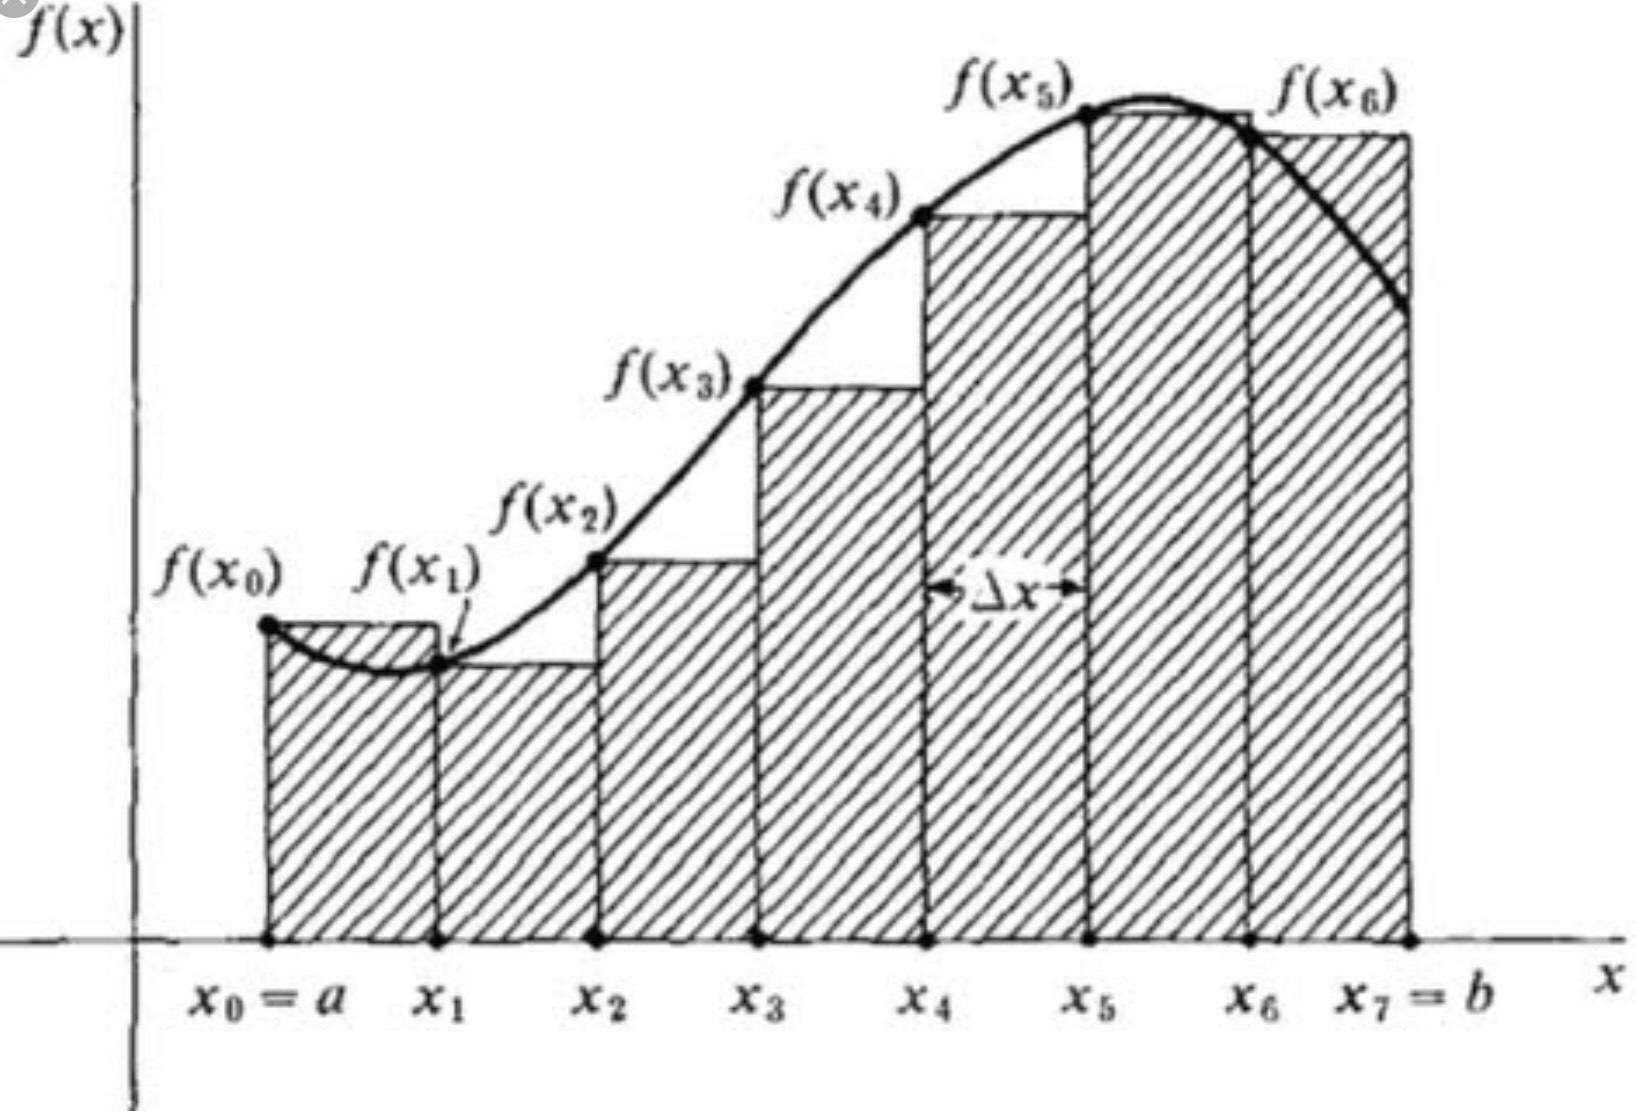
\includegraphics[width=\textwidth]{IMG_0380.jpg}
%		\hspace*{10pt}\hbox{\thinspace{\tiny\itshape vias.org}}
%		\caption{Single integration}
%	\end{subfigure}% 
%	~ 
%	\begin{subfigure}{0.48\textwidth}
%		
%		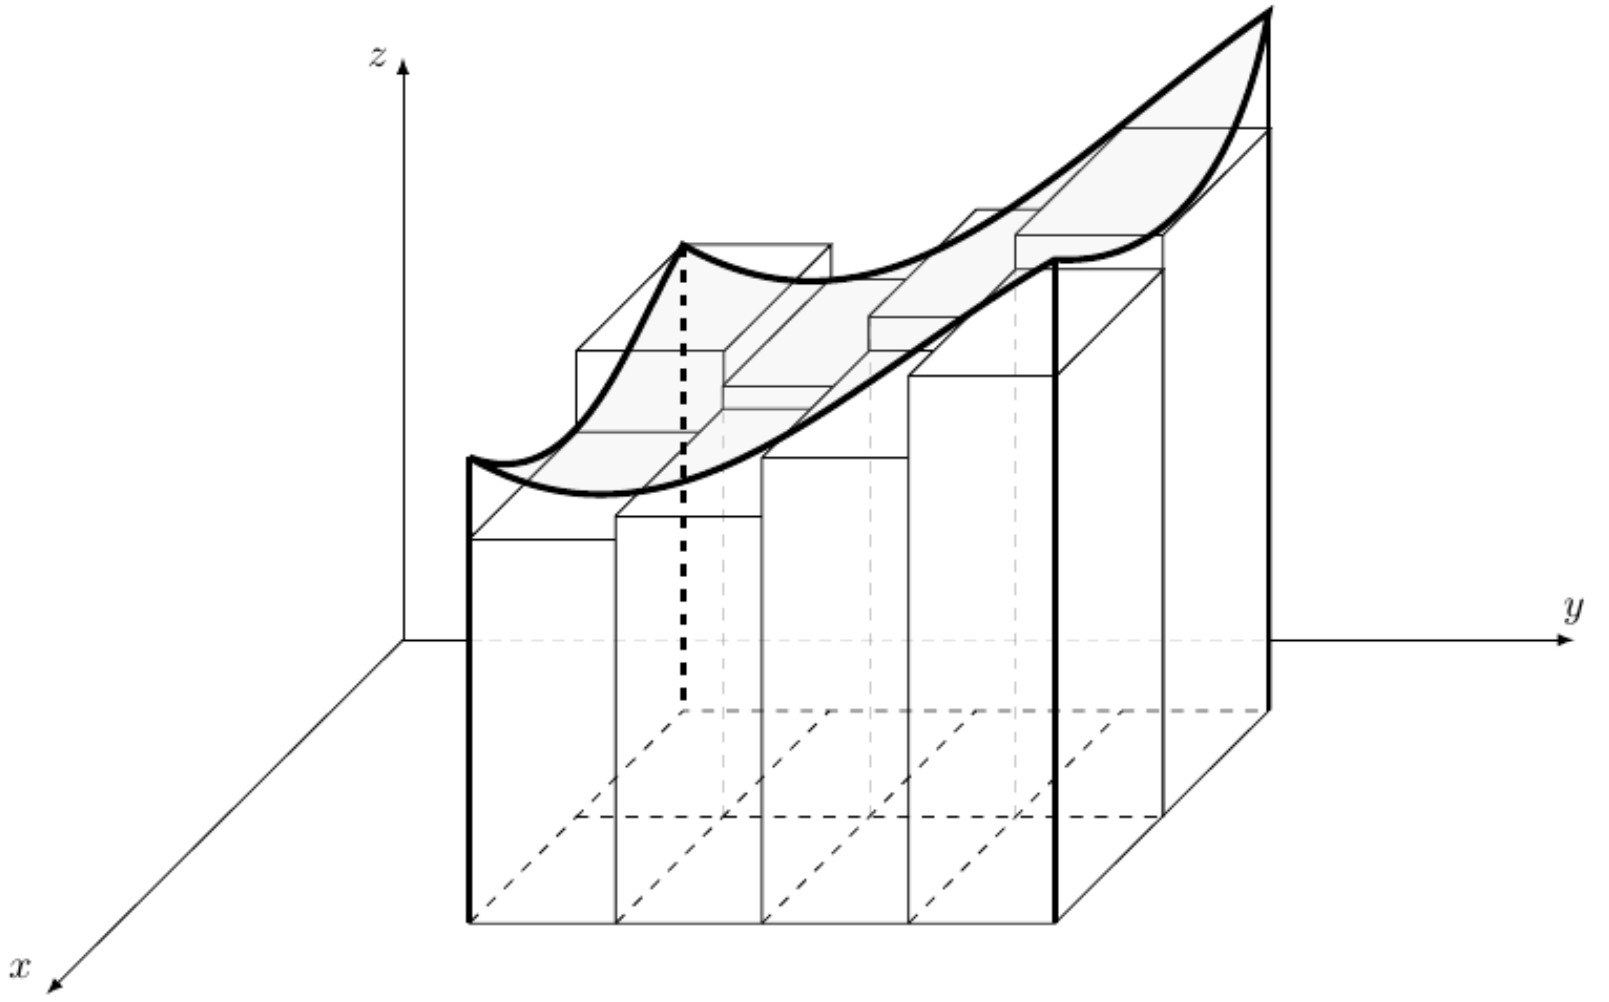
\includegraphics[width=\textwidth]{IMG_0385.jpg}
%		\hspace*{10pt}\hbox{\thinspace{\tiny\itshape tex.stackexchange.com}}
%		\caption{Double integration.}
%		\label{fig:2}
%	\end{subfigure}
%\end{figure}
%
%\end{frame}
%
%
%\begin{frame}
%\frametitle{Triple Integral}
%\begin{figure}
%	\centering
%	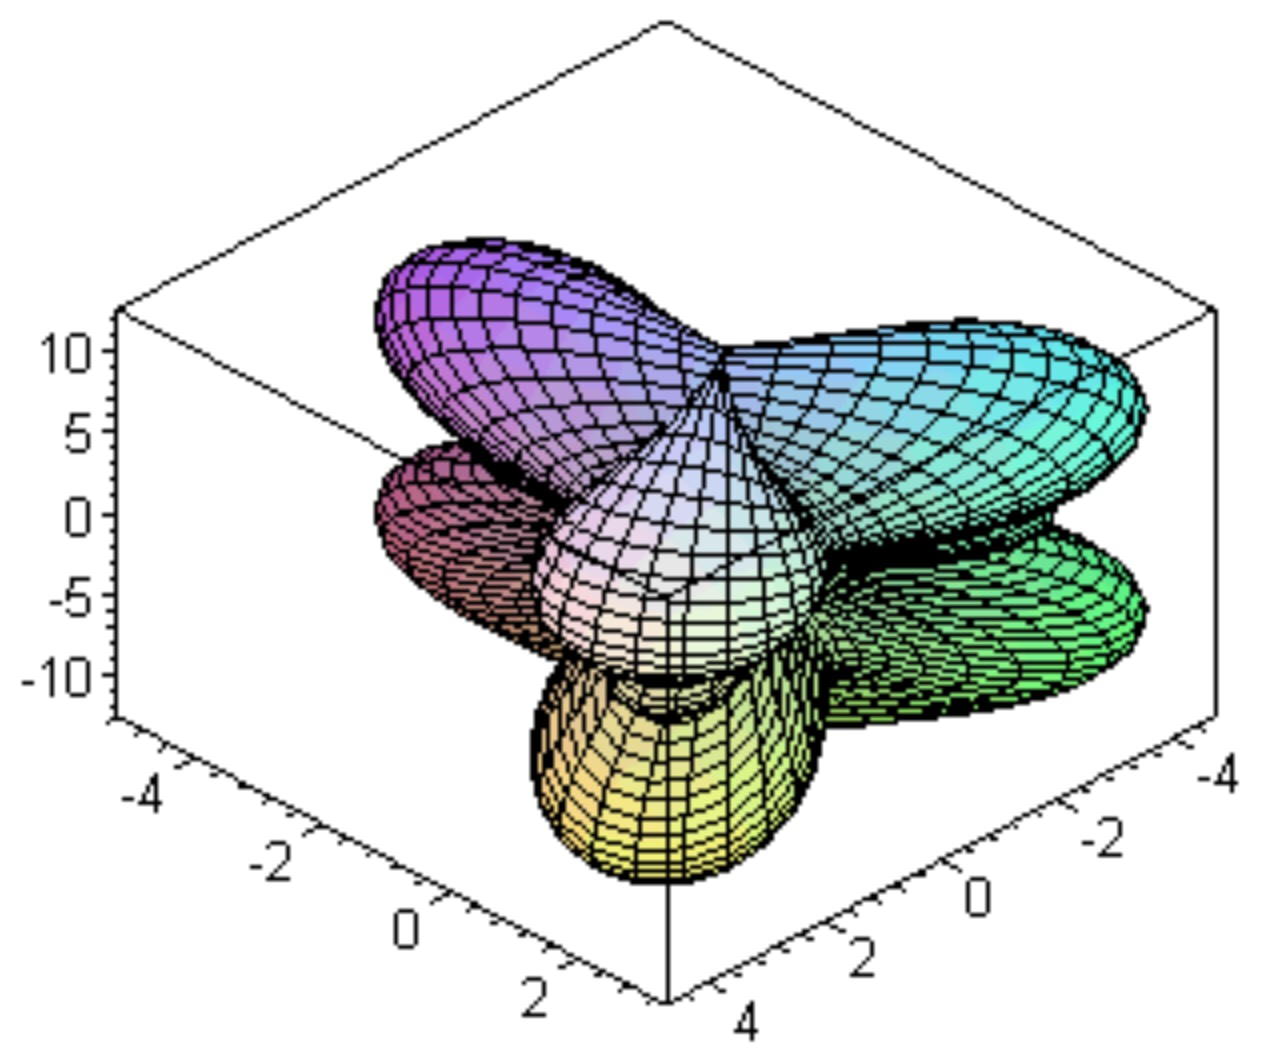
\includegraphics[height=.45\textheight]{IMG_0384.jpg}\\
%	\hspace*{10pt}\hbox{\thinspace{\tiny\itshape maplesoft.com}}
%\end{figure}
%
%$$\iiint\limits_{\mathbb{R}} F(x,y,z) dV = \int_{x=a}^{x=b} \int_{y=y_1(x)}^{y=y_2(x)} \int_{z=z_1(x,y)}^{z=z_2(x,y)} F(x,y,z) dz\,dy\,dx$$
%\textbf{Example:}
%\begin{itemize}
%	\item[(a)] $\int_0^1 \int_0^{1-x} \int_0^{2-x} xyz \,dz\,dy\,dx$
%\end{itemize}
%\end{frame}

\end{document}
